\documentclass{report}
\usepackage[utf8]{inputenc}
\usepackage[Bjornstrup]{fncychap}
\usepackage{graphicx}
\usepackage{amsmath}
\usepackage{amssymb}
\usepackage[spanish]{babel}
\usepackage{nicematrix}
\usepackage{apacite}

\bibliographystyle{apacite}
\selectlanguage{spanish}
{
  \setlength{\columnsep}{4mm}
  \setlength{\parindent}{0.5in}
  \setlength{\parskip}{1em}
  \renewcommand{\baselinestretch}{1.5}
  \setlength{\headheight}{33pt}

  \thispagestyle{empty}
			\begin{figure}[ht]
				\minipage{0.87\textwidth}
					 
\includegraphics[width=2cm]{fi.jpg}
					 \label{escudoFI}
				\endminipage
				\minipage{0.32\textwidth}
					 
\includegraphics[height = 2.25cm ,width=2cm]{unam.png}
					 \label{EscuoUNAM}
				 \endminipage
					 %%\vspace{-1cm}
			 \end{figure}
			 
			 \vspace{0.1cm}
			 
			 \begin{center}
				 {\scshape\LARGE \textbf{Universidad Nacional Autónoma de México} \par}
				 {\scshape\Large Facultad de Ingeniería\par}
				 
				  {\Large ESTRUCTURAS DE DATOS Y ALGORITMOS II}
	 
				 % Restauramos el interlineado:
				 \begin{center}
				 
				 {\LARGE \textit{Grupo: 07 - Semestre: 2024-1}}
	 
				 

				 {\LARGE\bfseries PROYECTO 2 – ALGORITMOS DE BÚSQUEDA\par}
	 
			 {\scshape\Large Fecha de entrega: 08/10/2023\par}	
	 
						 \LARGE	{ \textbf{Profesor:}}\\%% \textbf son negritas
			 \large		{ Edgar Tista Garcia}
			 
			 \vspace{-0.5cm}	
			 
			 \LARGE	{ \textbf{Alumno(s):}}\\%% \textbf son negritas
	 
			 \normalsize	 {Hernandez Gallardo Daniel Alonso}
			 
			 \vspace{-0.5cm}
			 
			 \normalsize		{Perez Osorio Luis Eduardo}
			 
			 \vspace{-0.5cm}
			 
			 \normalsize		{Valle Chavez Anton Yael}
			 
			 
	 %% \it es letra itálica
					 \vspace{1.25cm}
					 \vspace{0.9cm}
					 
				 \end{center}
		 
			 \end{center} 
}

\addto\captionsspanish{\renewcommand{\abstractname}{Abstract}}
\begin{document}





  

 


  \begin{abstract}

  \end{abstract}
    

 
  \section*{Resumen}
    Esta información presenta una aplicación sencilla de las transformaciones lineales en el estudio de la sincronización de sistemas físicos. Para comprender completamente la información presentada, se requiere cierto conocimiento teórico en el campo de las transformaciones lineales y la sincronización de sistemas físicos. Los conceptos clave incluyen las transformaciones lineales, sus propiedades, el concepto de núcleo o espacio nulo, la sincronización de sistemas, los grafos, los árboles de expansión dirigidos y las propiedades de la matriz Laplaciana. Estos conceptos brindan los fundamentos teóricos necesarios para comprender y analizar la aplicación de las transformaciones lineales en el estudio de la sincronización de sistemas físicos.

La sección de desarrollo incluye dos actividades. En la Actividad 1, se considera una red de 6 robots descrita por la segunda ley de Newton, y se presenta el grafo y la matriz de incidencia. Se calcula la matriz Laplaciana y se determinan sus valores propios y núcleo. En la Actividad 2, se analiza una red de 8 robots utilizando pasos similares. Se obtienen el grafo, la matriz de incidencia, la matriz Laplaciana, los valores propios y el núcleo. Se realizan simulaciones en MATLAB para visualizar la convergencia de los nodos en ambas actividades.

En general, esta información proporciona una demostración práctica del uso de las transformaciones lineales y los conceptos de teoría de grafos para estudiar la sincronización de sistemas físicos.



\tableofcontents

  

\chapter{Introducción} 
    \section*{Objetivo}
    Que el alumno desarrolle aplicaciones para la búsqueda por comparación de llaves y la
    transformación de llaves junto con la solución de colisiones
    \section*{investigación}
      \subsection*{Framework}
      Un framework es una agrupación de clases e interfaces que proporcionan una arquitectura lista para desarrollar software. Por ende, si se quiere implementar una nueva característica o clase, no es necesario definir un nuevo framework si ya existe uno. No obstante, una buena práctica en el paradigma orientado a objetos es incluir un framework con una colección de clases tal que todas las clases realicen el mismo tipo de operaciones.
      \subsection*{Colecciones en Java}
      Cualquier grupo de objetos individuales que se representa como una sola unidad se le conoce como una colección de objetos. En el lenguaje de programación Java, en Java Development Kit 1.2 se definió un modelo denominado Collection Framework que contiene todas las clases de colección con sus respectivas interfaces. De ahí que la interfaz de colección java.util.Collection y la interfaz de mapa java.util.Map son las dos interfaces principales de las clases de colección en Java.
      \subsection*{Collection Framework en Java}
      Antes de que existiera el Collection Framework, es decir, antes de JDK 1.2, los métodos estándar para agrupar objetos en Java, o colecciones, eran Arrays, Vectors o Hashtables. Todas estas colecciones no tenían una interfaz en común. Por consiguiente, aunque el objetivo principal de todas las colecciones es el mismo, la implementación de todas estas colecciones se definió de forma independiente y en consecuencia no había ninguna relación entre ellas. Además, era muy difícil para los programadores recordar los diferentes métodos, sintaxis y constructores existentes para cada clase de colección.
      \subsection*{Ventajas del Collection Framework en Java}
      Como ya se mencionó anteriormente, la falta de un framework dio lugar a las desventajas descritas en la sección anterior. Sin embargo, luego de que se declaró el framework se comenzaron a presentar ventajas.
      \begin{itemize}
          \item \textbf{API consistente:} la API tiene un conjunto básico de interfaces como Collection, Set, List o Map, donde todas las clases, ArrayList, LinkedList, Vector, que implementan estas interfaces tienen métodos en común.
          \item \textbf{Reduce la complejidad al programar:} un programador ya no tiene que preocuparse por el diseño de la Colección, lo cual le permite priorizar el resto de su programa. Por lo anterior, uno de los principales aspectos del paradigma orientado a objetos, el cual es abstracción se logró implementar satisfactoriamente.
          \item \textbf{Aumenta la eficiencia y la calidad del programa:} la eficiencia se ve incrementada gracias a la proporción de implementaciones de alto rendimiento para las estructuras de datos junto con algunos algoritmos útiles, ya que, en este caso, el programador no necesita preocuparse por elegir la mejor implementación de una estructura de datos particular. Simplemente puede utilizar la implementación predefinida y así aumentar el rendimiento de su algoritmo/programa.
      \end{itemize}
      \newpage
      \subsection*{Jerarquía del Collection Framework en Java}El paquete java.util contiene todas las clases e interfaces que requiere el Collection Framework. Asimismo, el Collection Framework contiene una interfaz conocida como Iterable, la cual proporciona un iterador para recorrer todas las colecciones. Todas las colecciones que amplían la interfaz, aumentan al mismo tiempo el rango del iterador y los métodos de esta. La siguiente imagen ilustra la jerarquía del Collection Framework.
    \begin{figure}[h]
    \centering
    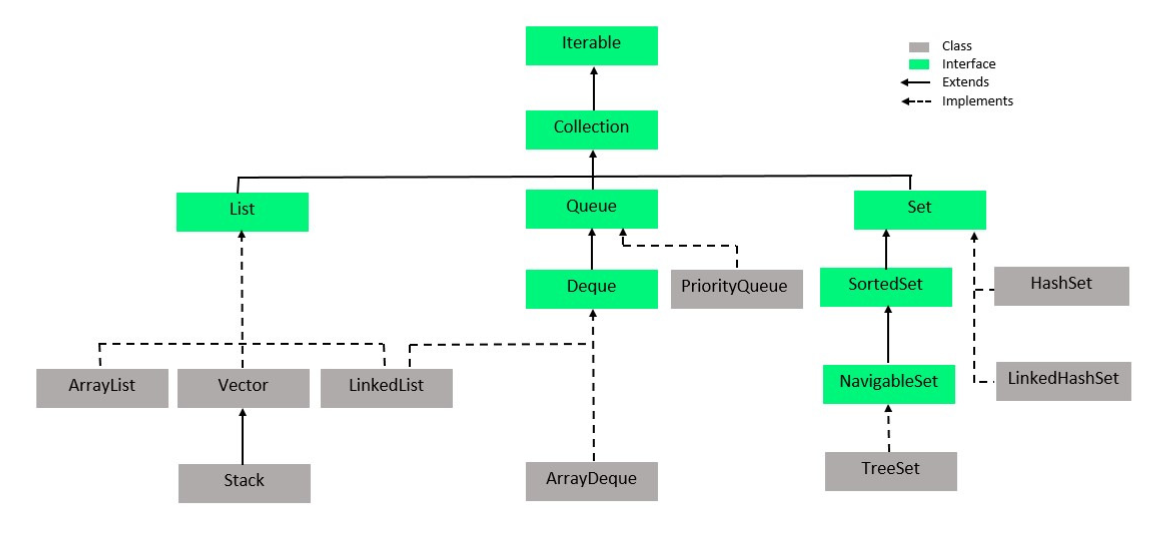
\includegraphics[width=1\linewidth]{Collection-Framework-1.png}
    \caption{GeeksforGeeks. (2023). Jerarquía del Collection Framework en Java[PNG].GeeksforGeeks.}
\end{figure}

\newpage
\chapter{Desarrollo}

\chapter{Conclusiones}
\textbf{Hernandez Gallardo Daniel Alonso} \\
\newpage
\textbf{Perez Osorio Luis Eduardo} \\

\newpage
\textbf{Valle Chavez Anton Yael} \\
\newpage
\nocite{*}
  \newpage
\bibliography{citas.bib}

\end{document}
